\section{Pruebas de Casos de Uso principales}
La aplicación móvil se compone de nueve vistas principales:
\begin{itemize}
 \item Configuración Personal
 \item Hoteles
 \item Vuelos
 \item Info AICM
 \item Lista de Equipaje
 \item Itinerario de viaje
 \item Ruta al AICM
 \item Ubícate
 \item Info Vuelo
\end{itemize}

A su vez cada módulo puede desplegar información diversa en otras vistas o en su caso a partir opciones adicionales sobre un menú 
secundario.
\clearpage

\subsection{Configuración Personal}

\definecolor{blanco}{RGB}{255,255,255}

\begin{table}[h]
	\begin{center}
		\begin{tabular}{|>{\color{blanco}}c|>{\color{blanco}}c|>{\color{blanco}}c|>{\color{blanco}}c|}
			\hline \rowcolor[RGB]{51,153,255} 
				{\bf CU} & 
				{\bf Acción o evento} &
				{\bf Resultados y/u observaciones} &
				{\bf } \\
			\hline 
				\multicolumn{1}{|m{1.8cm}|}{\centering CU-U-01} &
				\multicolumn{1}{m{4.5cm}|}{\centering Clic normal en crear configuración} &
				\multicolumn{1}{m{5.5cm}|}{\centering Se ingresan datos como email, clase de
				viaje y categoría de hotel por número de estrellas.El registro en el web service es exitoso.} &
				\multicolumn{1}{m{1.5cm}|}{\centering 
\includegraphics[width=8mm, height=8mm]{Figuras/palomita.png}} \\
      		\hline \rowcolor[RGB]{240,248,255} 
				\multicolumn{1}{|m{1.8cm}|}{\centering CU-U-01} &
				\multicolumn{1}{m{4.5cm}|}{\centering Clic normal en evitar configuración} &
				\multicolumn{1}{m{5.5cm}|}{\centering Se muestra el menú principal de TASMC y la opción de configurar sobre un 
				menú secundario.} &
				\multicolumn{1}{m{1.5cm}|}{\centering 
\includegraphics[width=8mm, height=8mm]{Figuras/palomita.png}} \\
		\hline 
				\multicolumn{1}{|m{1.8cm}|}{\centering CU-U-01} &
				\multicolumn{1}{m{4.4cm}|}{\centering Clic normal en opción de reconfiguración} &
				\multicolumn{1}{m{5.5cm}|}{\centering Se ingresan los datos de email, clase de viaje y categoría de 
				hotel. La fecha de configuración del usuario es modificada dentro del web service de administración.} &
				\multicolumn{1}{m{1.5cm}|}{\centering 
\includegraphics[width=8mm, height=8mm]{Figuras/palomita.png}} \\
      		\hline 
		\end{tabular}
	\end{center}
	\caption[Pruebas del módulo de Configuración Personal]{Pruebas del módulo de Configuración Personal} 
	\label{tab:pruebasConfiguracion}
\end{table}

\subsection{Hoteles}

\definecolor{blanco}{RGB}{255,255,255}

\begin{table}[h]
	\begin{center}
		\begin{tabular}{|>{\color{blanco}}c|>{\color{blanco}}c|>{\color{blanco}}c|>{\color{blanco}}c|}
			\hline \rowcolor[RGB]{51,153,255} 
				{\bf CU} & 
				{\bf Acción o evento} &
				{\bf Resultados y/u observaciones} &
				{\bf } \\
			\hline 
				\multicolumn{1}{|m{1.8cm}|}{\centering CU-U-02} &
				\multicolumn{1}{m{4.5cm}|}{\centering Clic normal en búsqueda de hoteles} &
				\multicolumn{1}{m{5.5cm}|}{\centering Despliega la información de hoteles correspondiente a las parámetros ingresados 
				en el formulario.} &
				\multicolumn{1}{m{1.5cm}|}{\centering 
\includegraphics[width=8mm, height=8mm]{Figuras/palomita.png}} \\
      		\hline \rowcolor[RGB]{240,248,255} 
				\multicolumn{1}{|m{1.8cm}|}{\centering CU-U-02} &
				\multicolumn{1}{m{4.5cm}|}{\centering Clic normal en detalle de hotel} &
				\multicolumn{1}{m{5.5cm}|}{\centering Muestra la información completa del hotel.} &
				\multicolumn{1}{m{1.5cm}|}{\centering 
\includegraphics[width=8mm, height=8mm]{Figuras/palomita.png}} \\
		\hline 
				\multicolumn{1}{|m{1.8cm}|}{\centering CU-U-02} &
				\multicolumn{1}{m{4.5cm}|}{\centering Clic normal en llamar hotel} &
				\multicolumn{1}{m{5.5cm}|}{\centering Activa el servicio de llamada hacia el número propio del hotel.} &
				\multicolumn{1}{m{1.5cm}|}{\centering 
\includegraphics[width=8mm, height=8mm]{Figuras/palomita.png}} \\
      		\hline \rowcolor[RGB]{240,248,255} 
				\multicolumn{1}{|m{1.8cm}|}{\centering CU-U-02} &
				\multicolumn{1}{m{4.5cm}|}{\centering Clic normal en página web del hotel} &
				\multicolumn{1}{m{5.5cm}|}{\centering Abre la página web propia del hotel en el navegador del teléfono.} &
				\multicolumn{1}{m{1.5cm}|}{\centering 
\includegraphics[width=8mm, height=8mm]{Figuras/palomita.png}} \\
      		        \hline 
      		        
		\end{tabular}
	\end{center}
	\caption[Pruebas del módulo de Hoteles]{Pruebas del módulo de Hoteles} 
	\label{tab:pruebasHoteles}
\end{table}
\clearpage

\subsection{Vuelos}

\definecolor{blanco}{RGB}{255,255,255}

\begin{table}[h]
	\begin{center}
		\begin{tabular}{|>{\color{blanco}}c|>{\color{blanco}}c|>{\color{blanco}}c|>{\color{blanco}}c|}
			\hline \rowcolor[RGB]{51,153,255} 
				{\bf CU} & 
				{\bf Acción o evento} &
				{\bf Resultados y/u observaciones} &
				{\bf } \\
			\hline 
				\multicolumn{1}{|m{1.8cm}|}{\centering CU-U-03} &
				\multicolumn{1}{m{4.5cm}|}{\centering Clic normal en búsqueda de vuelos} &
				\multicolumn{1}{m{5.5cm}|}{\centering Despliega la información correspondiente de vuelos según los parámetros ingresados 
				en el formulario.} &
				\multicolumn{1}{m{1.5cm}|}{\centering 
\includegraphics[width=8mm, height=8mm]{Figuras/palomita.png}} \\
			  \hline 
      		\end{tabular}
	\end{center}
	\caption[Pruebas del módulo de Vuelos]{Pruebas del módulo de Vuelos} 
	\label{tab:pruebasVuelos}
\end{table}

\subsection{Info AICM}

\definecolor{blanco}{RGB}{255,255,255}

\begin{table}[h]
	\begin{center}
		\begin{tabular}{|>{\color{blanco}}c|>{\color{blanco}}c|>{\color{blanco}}c|>{\color{blanco}}c|}
			\hline \rowcolor[RGB]{51,153,255} 
				{\bf CU} & 
				{\bf Acción o evento} &
				{\bf Resultados y/u observaciones} &
				{\bf } \\
			\hline 
				\multicolumn{1}{|m{1.8cm}|}{\centering CU-U-04} &
				\multicolumn{1}{m{4.5cm}|}{\centering Clic normal en Info AICM} &
				\multicolumn{1}{m{5.5cm}|}{\centering Despliega la información del AICM como sitio web, teléfono, ubicación, y dos botones para 
				el mapa y los servicios.} &
				\multicolumn{1}{m{1.5cm}|}{\centering 
\includegraphics[width=8mm, height=8mm]{Figuras/palomita.png}} \\
      		\hline \rowcolor[RGB]{240,248,255} 
      				\multicolumn{1}{|m{1.8cm}|}{\centering CU-U-04} &
				\multicolumn{1}{m{4.5cm}|}{\centering Clic normal en mapa de AICM} &
				\multicolumn{1}{m{5.5cm}|}{\centering Se muestra una vista dividida en planta baja y alta, la cuál 
				puede ser intercambiada mediante un deslizamiento en la pantalla de izquierda a derecha.} &
				\multicolumn{1}{m{1.5cm}|}{\centering 
\includegraphics[width=8mm, height=8mm]{Figuras/palomita.png}} \\
		\hline 
				\multicolumn{1}{|m{1.8cm}|}{\centering CU-U-04} &
				\multicolumn{1}{m{4.5cm}|}{\centering Clic normal en servicios del AICM} &
				\multicolumn{1}{m{5.5cm}|}{\centering Se una lista de los servicios que ofrece el AICM-T1.} &
				\multicolumn{1}{m{1.5cm}|}{\centering 
\includegraphics[width=8mm, height=8mm]{Figuras/palomita.png}} \\
      		        \hline 
    		\end{tabular}
	\end{center}
	\caption[Pruebas del módulo de Info AICM]{Pruebas del módulo de Info AICM} 
	\label{tab:pruebasInfoAICM}
\end{table}

\clearpage

\subsection{Lista de Equipaje}

\definecolor{blanco}{RGB}{255,255,255}

\begin{table}[h]
	\begin{center}
		\begin{tabular}{|>{\color{blanco}}c|>{\color{blanco}}c|>{\color{blanco}}c|>{\color{blanco}}c|}
			\hline \rowcolor[RGB]{51,153,255} 
				{\bf CU} & 
				{\bf Acción o evento} &
				{\bf Resultados y/u observaciones} &
				{\bf } \\
			\hline 
				\multicolumn{1}{|m{1.8cm}|}{\centering CU-U-05} &
				\multicolumn{1}{m{4.5cm}|}{\centering Clic normal en Lista de Equipaje} &
				\multicolumn{1}{m{5.5cm}|}{\centering Se despliega una lista de equipajes los cuales pueden ser sugerencias 
				cargadas directamente desde el web service o listas creadas por el usuario. Se muestra un mensaje solicitando al usuario 
				conectarse a internet en caso de no tener encendido ese servicio. No carga las sugerencias de equipajes 
				si no se encuentra conectado a internet.} &
				\multicolumn{1}{m{1.5cm}|}{\centering 
\includegraphics[width=8mm, height=8mm]{Figuras/palomita.png}} \\
      		\hline \rowcolor[RGB]{240,248,255} 
      				\multicolumn{1}{|m{1.8cm}|}{\centering CU-U-05} &
				\multicolumn{1}{m{4.5cm}|}{\centering Clic normal en botón de nuevo equipaje} &
				\multicolumn{1}{m{5.5cm}|}{\centering Se muestra un vista donde se debe ingresar un nombre para la lista de 
				equipaje asi como una lista con los objetos que desee llevar en su viaje.} &
				\multicolumn{1}{m{1.5cm}|}{\centering 
\includegraphics[width=8mm, height=8mm]{Figuras/palomita.png}} \\
		\hline 
				\multicolumn{1}{|m{1.8cm}|}{\centering CU-U-05} &
				\multicolumn{1}{m{4.5cm}|}{\centering Clic normal en lista de equipaje} &
				\multicolumn{1}{m{5.5cm}|}{\centering Se muestran una lista con los objetos en el equipaje, mediante 
				la cuál es posible verificar los mismos a la hora de viajar.} &
				\multicolumn{1}{m{1.5cm}|}{\centering 
\includegraphics[width=8mm, height=8mm]{Figuras/palomita.png}} \\
		\hline \rowcolor[RGB]{240,248,255} 
      				\multicolumn{1}{|m{1.8cm}|}{\centering CU-U-05} &
				\multicolumn{1}{m{4.5cm}|}{\centering Clic normal en editar equipaje} &
				\multicolumn{1}{m{5.5cm}|}{\centering Se muestra un vista donde es posible agregar o eliminar objetos del equipaje.} &
				\multicolumn{1}{m{1.5cm}|}{\centering 
\includegraphics[width=8mm, height=8mm]{Figuras/palomita.png}} \\
		\hline 
		      		              		        
    		\end{tabular}
	\end{center}
	\caption[Pruebas del módulo Lista de Equipaje]{Pruebas del módulo Lista de Equipaje} 
	\label{tab:pruebasEquipaje}
\end{table}

\clearpage

\subsection{Itinerario de viaje}

\definecolor{blanco}{RGB}{255,255,255}

\begin{table}[h]
	\begin{center}
		\begin{tabular}{|>{\color{blanco}}c|>{\color{blanco}}c|>{\color{blanco}}c|>{\color{blanco}}c|}
			\hline \rowcolor[RGB]{51,153,255} 
				{\bf CU} & 
				{\bf Acción o evento} &
				{\bf Resultados y/u observaciones} &
				{\bf } \\
			\hline 
				\multicolumn{1}{|m{1.8cm}|}{\centering CU-U-06} &
				\multicolumn{1}{m{4.5cm}|}{\centering Clic normal en itinerario de Viaje} &
				\multicolumn{1}{m{5.5cm}|}{\centering Se despliega una lista de itinerarios con los itinerarios creados por el usuario, 
				cada uno con información referente al destino y actividades en dicho viaje.} &
				\multicolumn{1}{m{1.5cm}|}{\centering 
\includegraphics[width=8mm, height=8mm]{Figuras/palomita.png}} \\
      		\hline \rowcolor[RGB]{240,248,255} 
      				\multicolumn{1}{|m{1.8cm}|}{\centering CU-U-06} &
				\multicolumn{1}{m{4.5cm}|}{\centering Clic normal sobre un itinerario} &
				\multicolumn{1}{m{5.5cm}|}{\centering Se muestran los detalles del itinerario como es el destino y las actividades a realizar, 
				mismo que puede ser editado.} &
				\multicolumn{1}{m{1.5cm}|}{\centering 
\includegraphics[width=8mm, height=8mm]{Figuras/palomita.png}} \\
		\hline 
				\multicolumn{1}{|m{1.8cm}|}{\centering CU-U-06} &
				\multicolumn{1}{m{4.5cm}|}{\centering Clic normal en nuevo itinerario} &
				\multicolumn{1}{m{5.5cm}|}{\centering Se solicitan los datos del itinerario como es el destino y las 
				actividades a realizar. El itinerario es guardado correctamente en la base de datos.} &
				\multicolumn{1}{m{1.5cm}|}{\centering 
\includegraphics[width=8mm, height=8mm]{Figuras/palomita.png}} \\
		\hline \rowcolor[RGB]{240,248,255} 
      				\multicolumn{1}{|m{1.8cm}|}{\centering CU-U-06} &
				\multicolumn{1}{m{4.5cm}|}{\centering Arrastrar itinerario para eliminación} &
				\multicolumn{1}{m{5.5cm}|}{\centering Se deja presionado el itinerario y se arrastra hacia la derecha para 
				su eliminación. Se elimina correctamente de la base de datos.} &
				\multicolumn{1}{m{1.5cm}|}{\centering 
\includegraphics[width=8mm, height=8mm]{Figuras/palomita.png}} \\
		\hline 
		      		              		        
    		\end{tabular}
    	\end{center}
	\caption[Pruebas del módulo de Itinerario]{Pruebas del módulo de Itinerario} 
	\label{tab:pruebasItinerario}
\end{table}

\subsection{Ruta al AICM}

\definecolor{blanco}{RGB}{255,255,255}

\begin{table}[h]
	\begin{center}
		\begin{tabular}{|>{\color{blanco}}c|>{\color{blanco}}c|>{\color{blanco}}c|>{\color{blanco}}c|}
			\hline \rowcolor[RGB]{51,153,255} 
				{\bf CU} & 
				{\bf Acción o evento} &
				{\bf Resultados y/u observaciones} &
				{\bf } \\
			\hline 
				\multicolumn{1}{|m{1.8cm}|}{\centering CU-U-07} &
				\multicolumn{1}{m{4.5cm}|}{\centering Clic normal en Ruta AICM} &
				\multicolumn{1}{m{5.5cm}|}{\centering Se despliega un mapa con las distintas localidades de las terminales del AICM. 
				Así como la opción de localización actual.} &
				\multicolumn{1}{m{1.5cm}|}{\centering 
\includegraphics[width=8mm, height=8mm]{Figuras/palomita.png}} \\
      		\hline \rowcolor[RGB]{240,248,255} 
      				\multicolumn{1}{|m{1.8cm}|}{\centering CU-U-07} &
				\multicolumn{1}{m{4.5cm}|}{\centering Clic normal sobre marcador de localidades(origen-destino) para generar la ruta} &
				\multicolumn{1}{m{5.5cm}|}{\centering Se marcan los dos puntos mediante marcadores entre los cuales se quiere generar la ruta. 
				La ruta se genera exitosamente. No es posible generar la ruta sin una conexión a internet.} &
				\multicolumn{1}{m{1.5cm}|}{\centering 
\includegraphics[width=8mm, height=8mm]{Figuras/palomita.png}} \\
		\hline 
    	\end{tabular}
	\end{center}
	\caption[Pruebas del módulo Ruta al AICM]{Pruebas del módulo Ruta al AICM} 
	\label{tab:pruebasRuta}
\end{table}

\clearpage

\subsection{Ubícate}

\definecolor{blanco}{RGB}{255,255,255}

\begin{table}[h]
	\begin{center}
		\begin{tabular}{|>{\color{blanco}}c|>{\color{blanco}}c|>{\color{blanco}}c|>{\color{blanco}}c|}
			\hline \rowcolor[RGB]{51,153,255} 
				{\bf CU} & 
				{\bf Acción o evento} &
				{\bf Resultados y/u observaciones} &
				{\bf } \\
			\hline 
				\multicolumn{1}{|m{1.8cm}|}{\centering CU-U-08} &
				\multicolumn{1}{m{4.5cm}|}{\centering Clic normal en Ubicate} &
				\multicolumn{1}{m{5.5cm}|}{\centering Se muestra un mapa del interior del aeropuerto el cuál ayudará a localizar 
				de manera más rápida. El mapa podrá ser intercambiado mediante un menú secundario.} &
				\multicolumn{1}{m{1.5cm}|}{\centering 
\includegraphics[width=8mm, height=8mm]{Figuras/palomita.png}} \\
      		\hline 
    	\end{tabular}
	\end{center}
	\caption[Pruebas del módulo Ubicate]{Pruebas del módulo Ubicate} 
	\label{tab:pruebasUbicate}
\end{table}

\subsection{Info Vuelo}

\definecolor{blanco}{RGB}{255,255,255}

\begin{table}[h]
	\begin{center}
		\begin{tabular}{|>{\color{blanco}}c|>{\color{blanco}}c|>{\color{blanco}}c|>{\color{blanco}}c|}
			\hline \rowcolor[RGB]{51,153,255} 
				{\bf CU} & 
				{\bf Acción o evento} &
				{\bf Resultados y/u observaciones} &
				{\bf } \\
			\hline 
				\multicolumn{1}{|m{1.8cm}|}{\centering CU-U-09} &
				\multicolumn{1}{m{4.5cm}|}{\centering Clic normal Info Vuelo} &
				\multicolumn{1}{m{5.5cm}|}{\centering Se muestra la información de vuelos dividida por salidas y 
				llegadas nacionales e internacionales, las cuales podrán ser visualizadas detalladamente mediante un 
				deslizamiento en la pantalla.} &
				\multicolumn{1}{m{1.5cm}|}{\centering 
\includegraphics[width=8mm, height=8mm]{Figuras/palomita.png}} \\
      		\hline \rowcolor[RGB]{240,248,255} 
      				\multicolumn{1}{|m{1.8cm}|}{\centering CU-U-07} &
				\multicolumn{1}{m{4.5cm}|}{\centering Clic normal en buscar vuelo} &
				\multicolumn{1}{m{5.5cm}|}{\centering Se debe ingresar el número propio del vuelo del usuario, 
				posteriormente se visualizará la información referente al mismo.} &
				\multicolumn{1}{m{1.5cm}|}{\centering 
\includegraphics[width=8mm, height=8mm]{Figuras/palomita.png}} \\
		\hline 
    	\end{tabular}
	\end{center}
	\caption[Pruebas del módulo Info Vuelo]{Pruebas del módulo Info Vuelo} 
	\label{tab:pruebasInfoVuelo}
\end{table}
\clearpage

\section{Pruebas Aplicación móvil TASMC}

\subsection{Obtención de rutas}
A continuación se presentan dos escenarios distintos sobre la generación de rutas hacia las dos terminales del AICM en particular 
a partir de la ubicación actual del usuario. En cada uno de los escenarios a sido seleccionada la opción de ubicación actual, 
a partir de eso se pone un marcador en dicha ubicación y mediante el botón de Ir a AICM se puede obtener la ubicación de las dos 
terminales con las que cuenta el AICM donde posteriormente quedará fijado el marcador de la siguiente localidad y a partir de ello 
generar la ruta.

\begin{figure}[h]
	\centering
		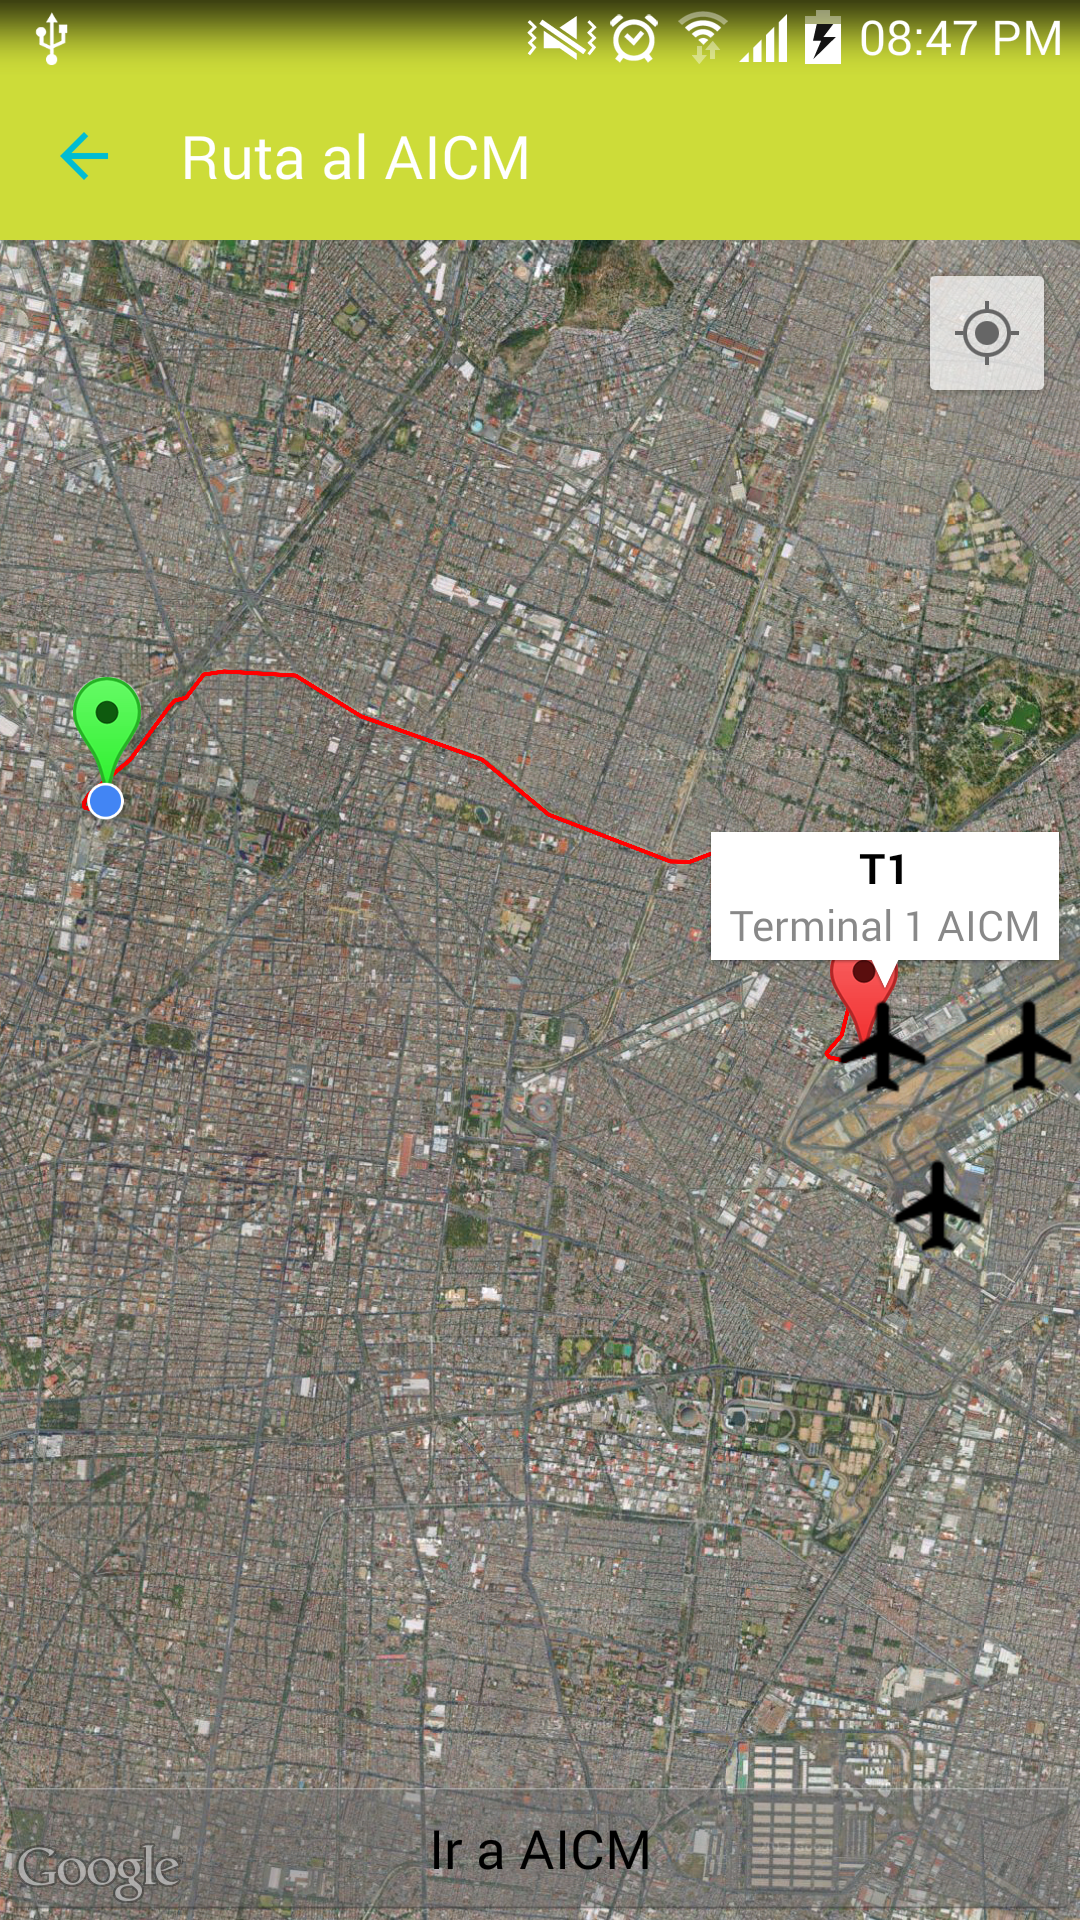
\includegraphics[width=0.5\textwidth]{Figuras/escenariot1.png}
		\rule{30em}{0.5pt}
	\caption[Escenario de prueba 1 para la generación de ruta (Terminal 1)]{Escenario de prueba 1 para la generación de ruta (Terminal 1)}
	\label{fig:vistaPruebaR1}
\end{figure}
\clearpage

\begin{figure}[h]
	\centering
		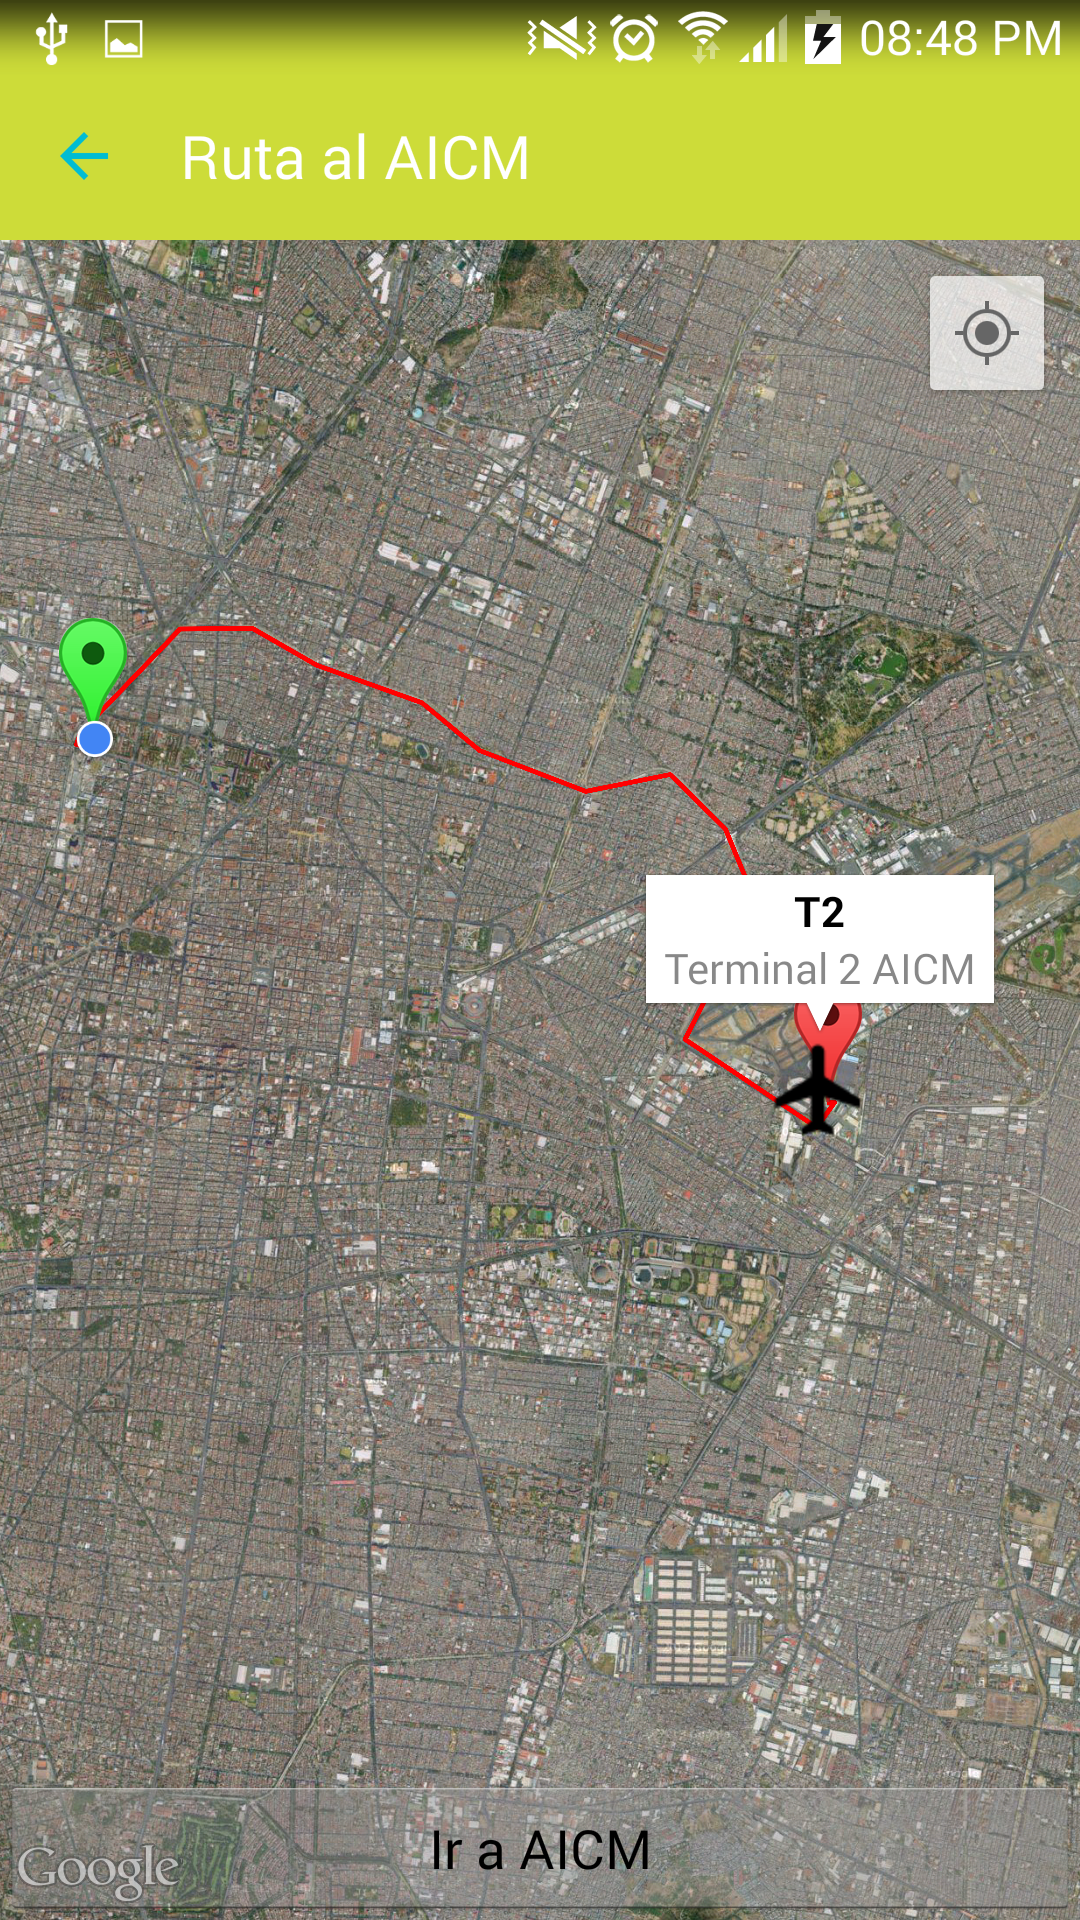
\includegraphics[width=0.5\textwidth]{Figuras/escenariot2.png}
		\rule{30em}{0.5pt}
	\caption[Escenario de prueba 2 para la generación de ruta (Terminal 2)]{Escenario de prueba 2 para la generación de ruta (Terminal 2)}
	\label{fig:vistaPruebaR2}
\end{figure}
\clearpage

\subsection{Pruebas de trayectorias para la localización dentro del AICM}
Para probar el módulo de ubicate se realizaron un trazado de distintos tipos de trayectorias donde se analizó cual fue la mejor 
opción en cuestión de exactitud. 

\subsection{Trayectoria redundante}
Se trazo una trayectoria redundante con la finalidad de tener un camino que fuera de ida y vuelta. Los resultados que se obtuvieron 
fueron negativos ya que se tenía pensado que fuera redundante y se pudiera usar una trayectoria tanto de ida como vuelta.

\begin{figure}[h]
	\centering
		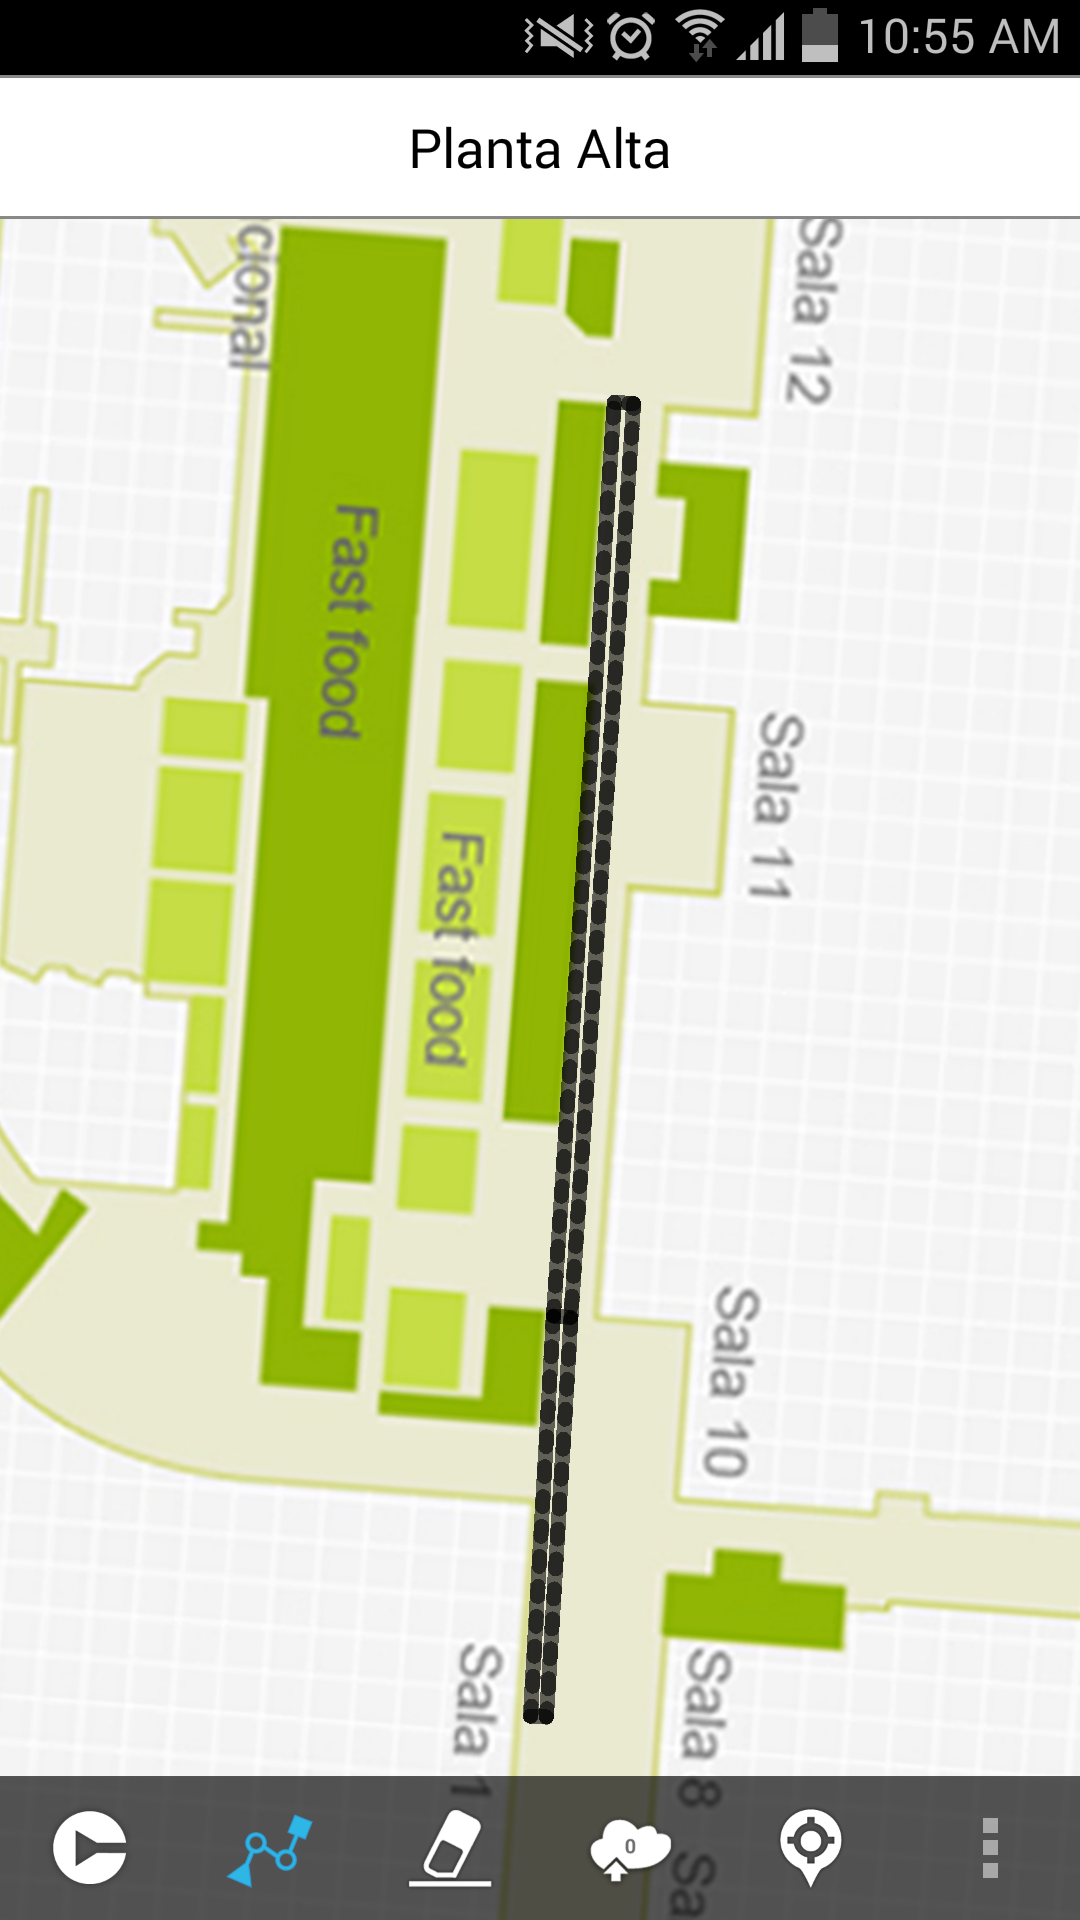
\includegraphics[width=0.5\textwidth]{Figuras/redundante.png}
		\rule{30em}{0.5pt}
	\caption[Prueba trayectoria redundante]{Prueba trayectoria redundante}
	\label{fig:vistaPruebaRedundante}
\end{figure}
\clearpage

\subsection{Trayectoria zigzag}
Se trazo una trayectoria simulando un zigzag la cual no fue efectiva pues a pesar de abarcar más área, el API utilizada guarda unicamente 
la trayectoria, no los valores magnéticos en el área.
\begin{figure}[h]
	\centering
		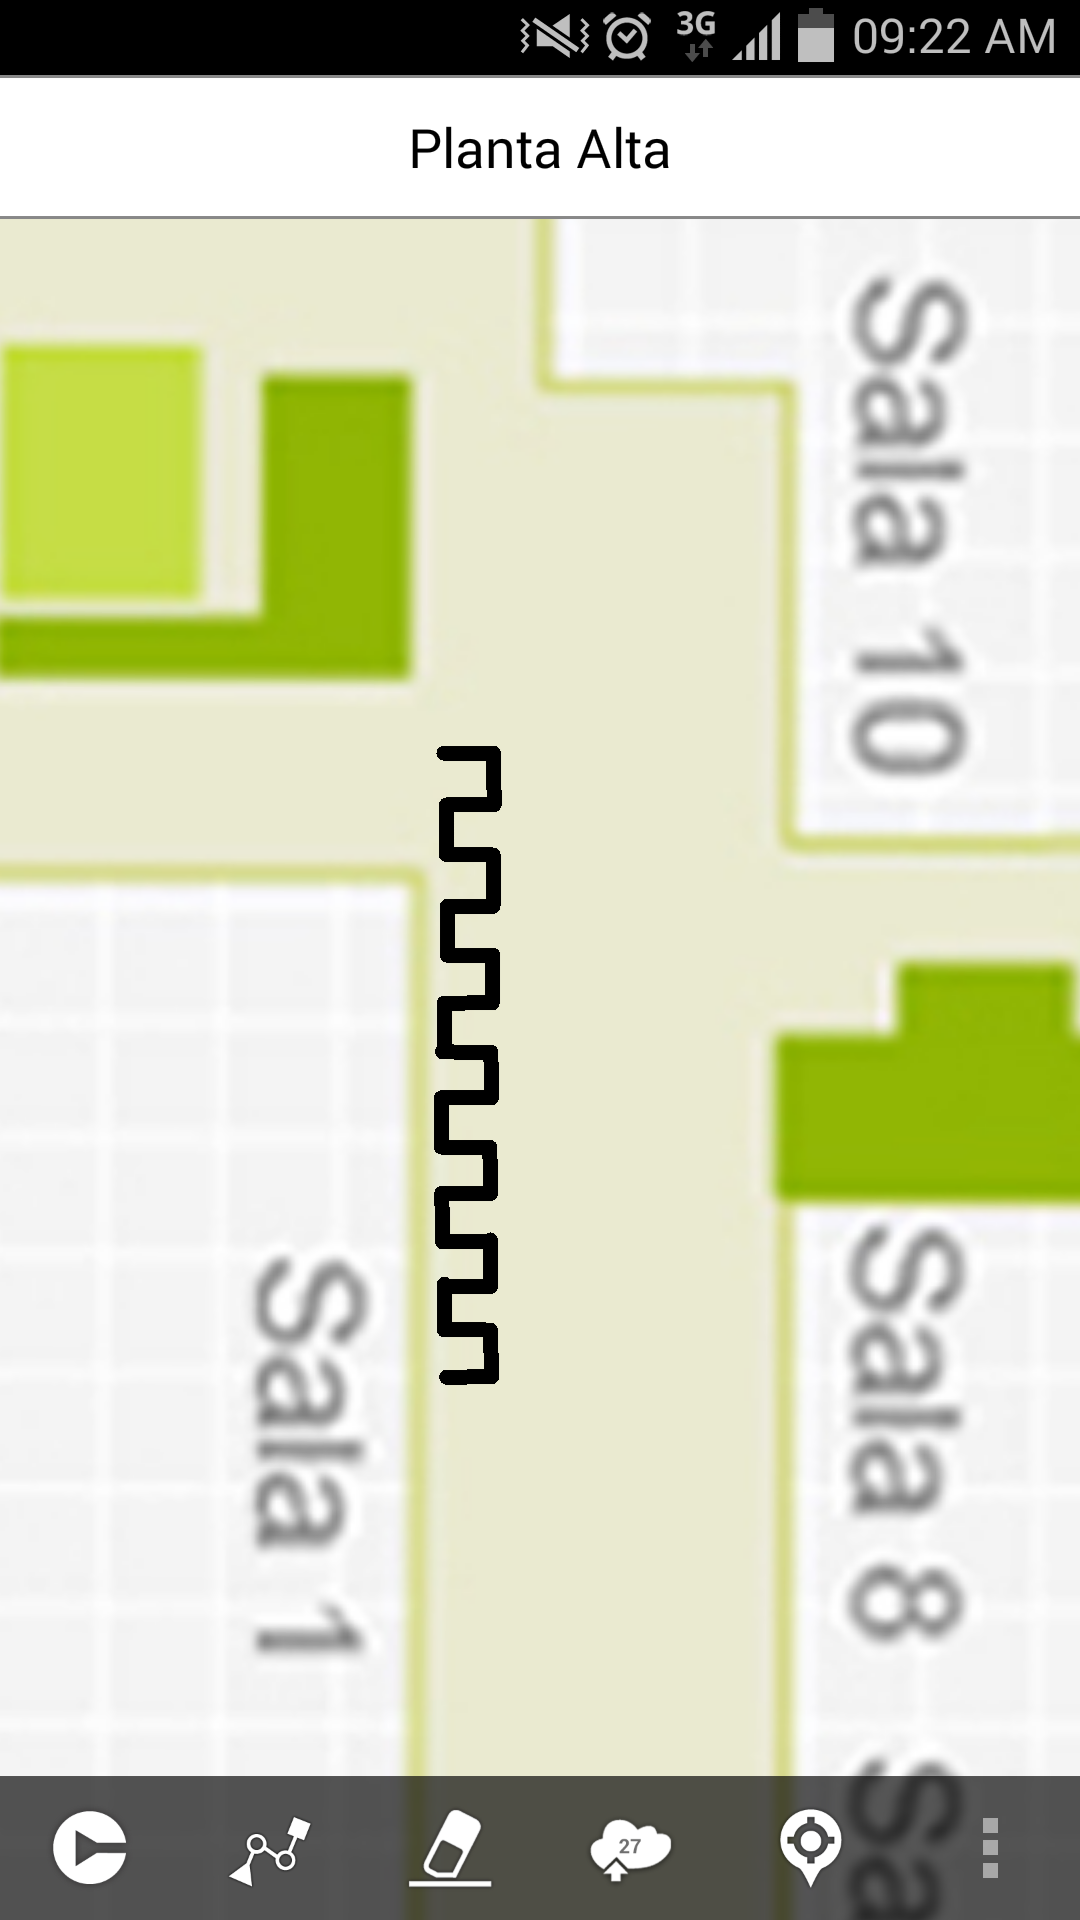
\includegraphics[width=0.5\textwidth]{Figuras/zigzag.png}
		\rule{30em}{0.5pt}
	\caption[Prueba trayectoria zigzag]{Prueba trayectoria zigzag}
	\label{fig:vistaPruebaZig}
\end{figure}
\clearpage

\subsection{Trayectoria medio backbone}
Se trazo únicamente una ruta la cual serviría de ida y vuelta, se dividio el andén de pasajeros a la mitad pensando que teniendo 
trayectorias segmentadas por cada sala de última espera se podía obtener una mayor exactitud pero los resultados eran de cinco metros, lo cual no es tan aceptable en la localización en interiores.
\begin{figure}[h]
	\centering
		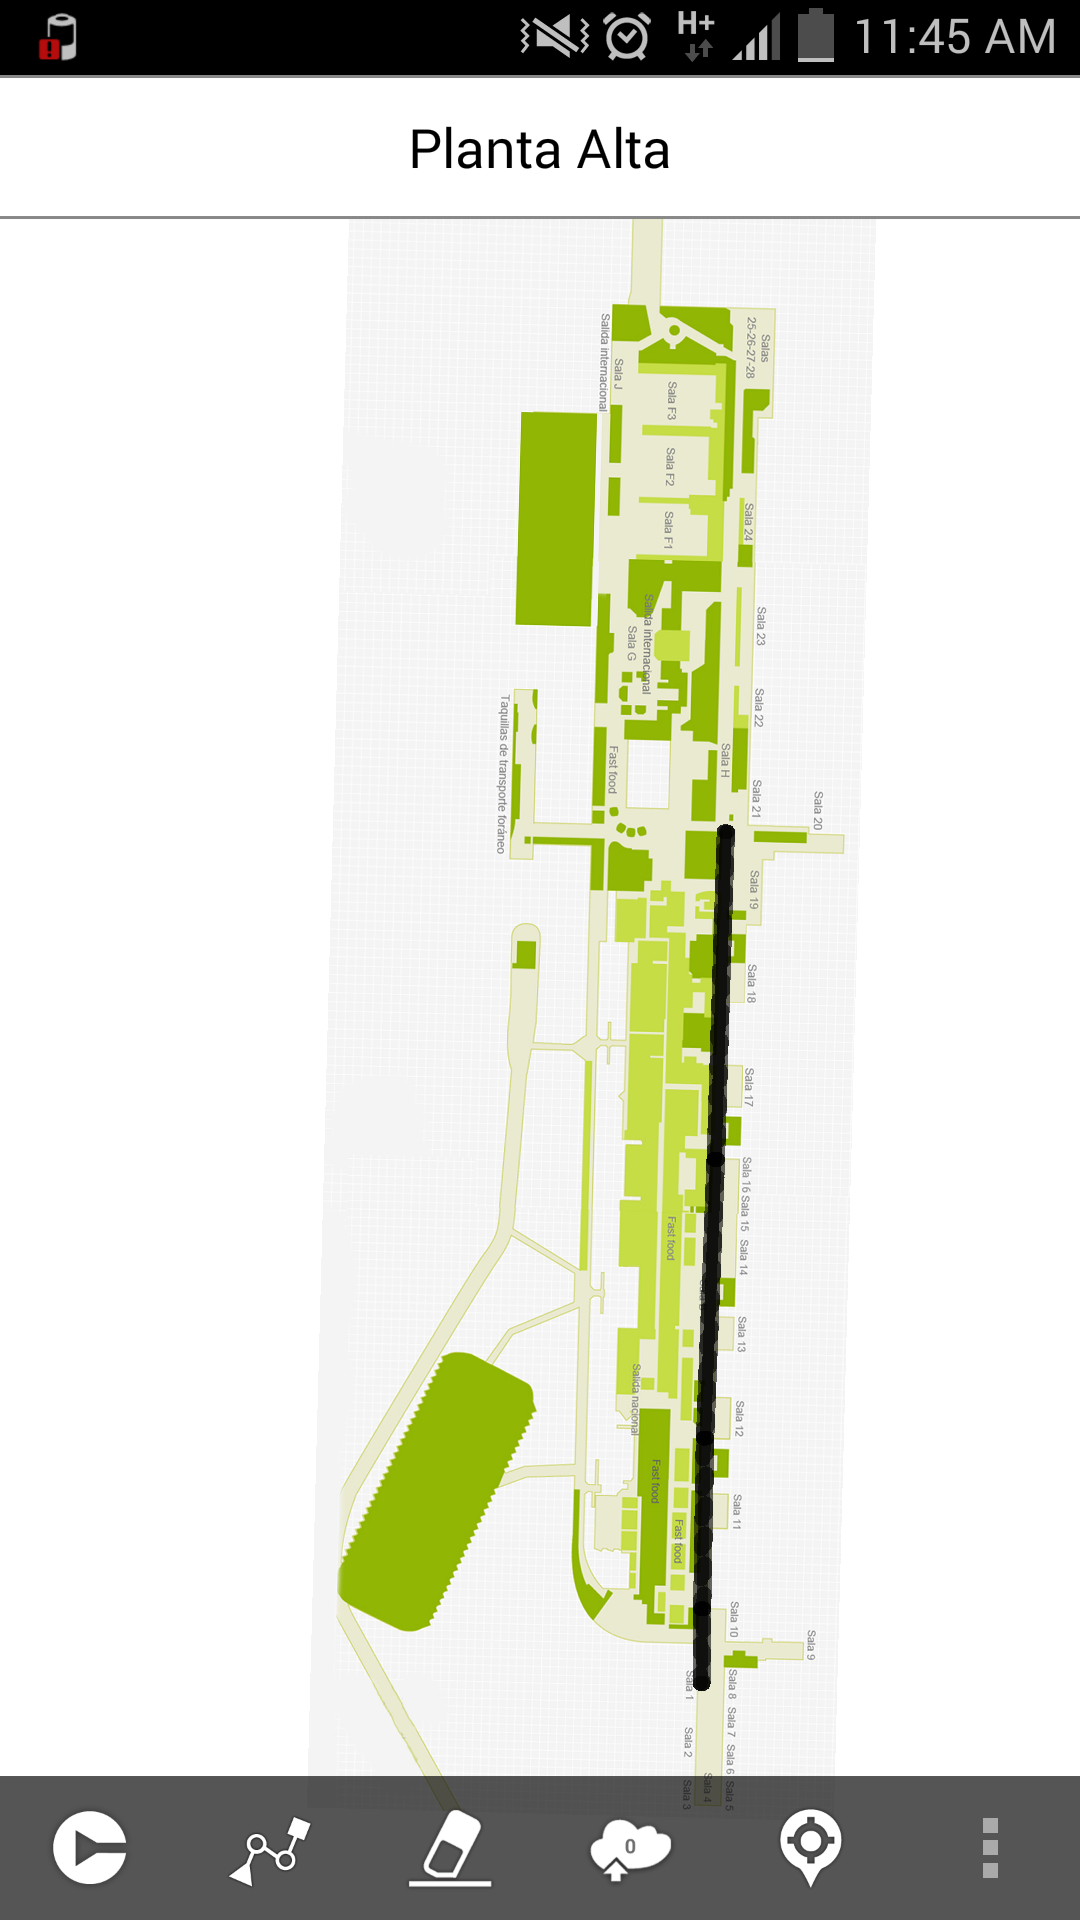
\includegraphics[width=0.5\textwidth]{Figuras/medioback.png}
		\rule{30em}{0.5pt}
	\caption[Prueba trayectoria medio backbone]{Prueba trayectoria medio backbone}
	\label{fig:vistaPruebaMedioBack}
\end{figure}
\clearpage

\subsection{Trayectoria backbone}
Finalmente se trazó un llamado backbone sobre el anden principal de pasajeros, medio por el cual se comunican las distintas salas de espera 
del AICM-T1 de está manera se obtuvieron los mejores resutados ya que se pudo obtener una exactitud de tres metros. La trayectoria backbone se considera la técnica mas adecuada para desarrollar la localización en interiores. A partir de ésta técnica se trazaron las distintas trayectorias en cada una de las salas de última espera.
\begin{figure}[h]
	\centering
		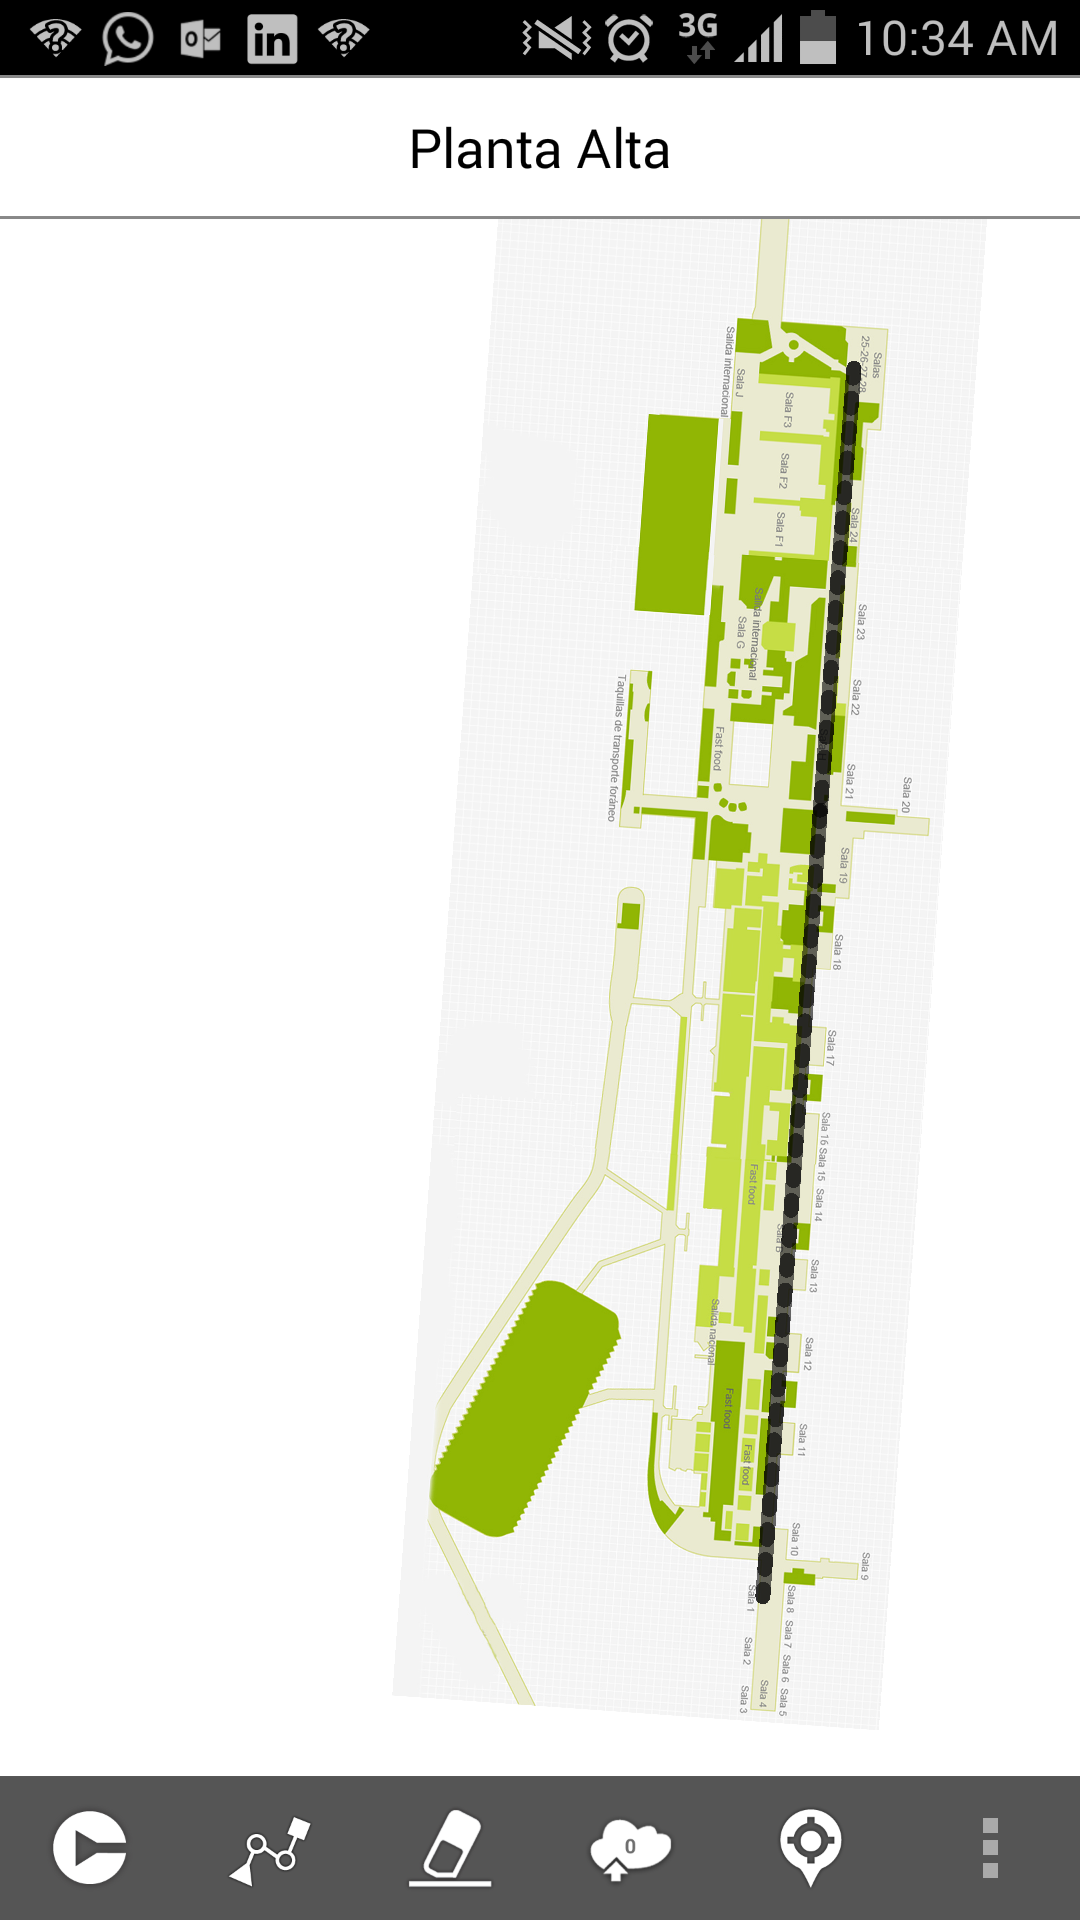
\includegraphics[width=0.5\textwidth]{Figuras/backbone.png}
		\rule{30em}{0.5pt}
	\caption[Prueba trayectoria backbone]{Prueba trayectoria backbone}
	\label{fig:vistaPruebaBackbone}
\end{figure}
\clearpage

\begin{figure}[h]
	\centering
		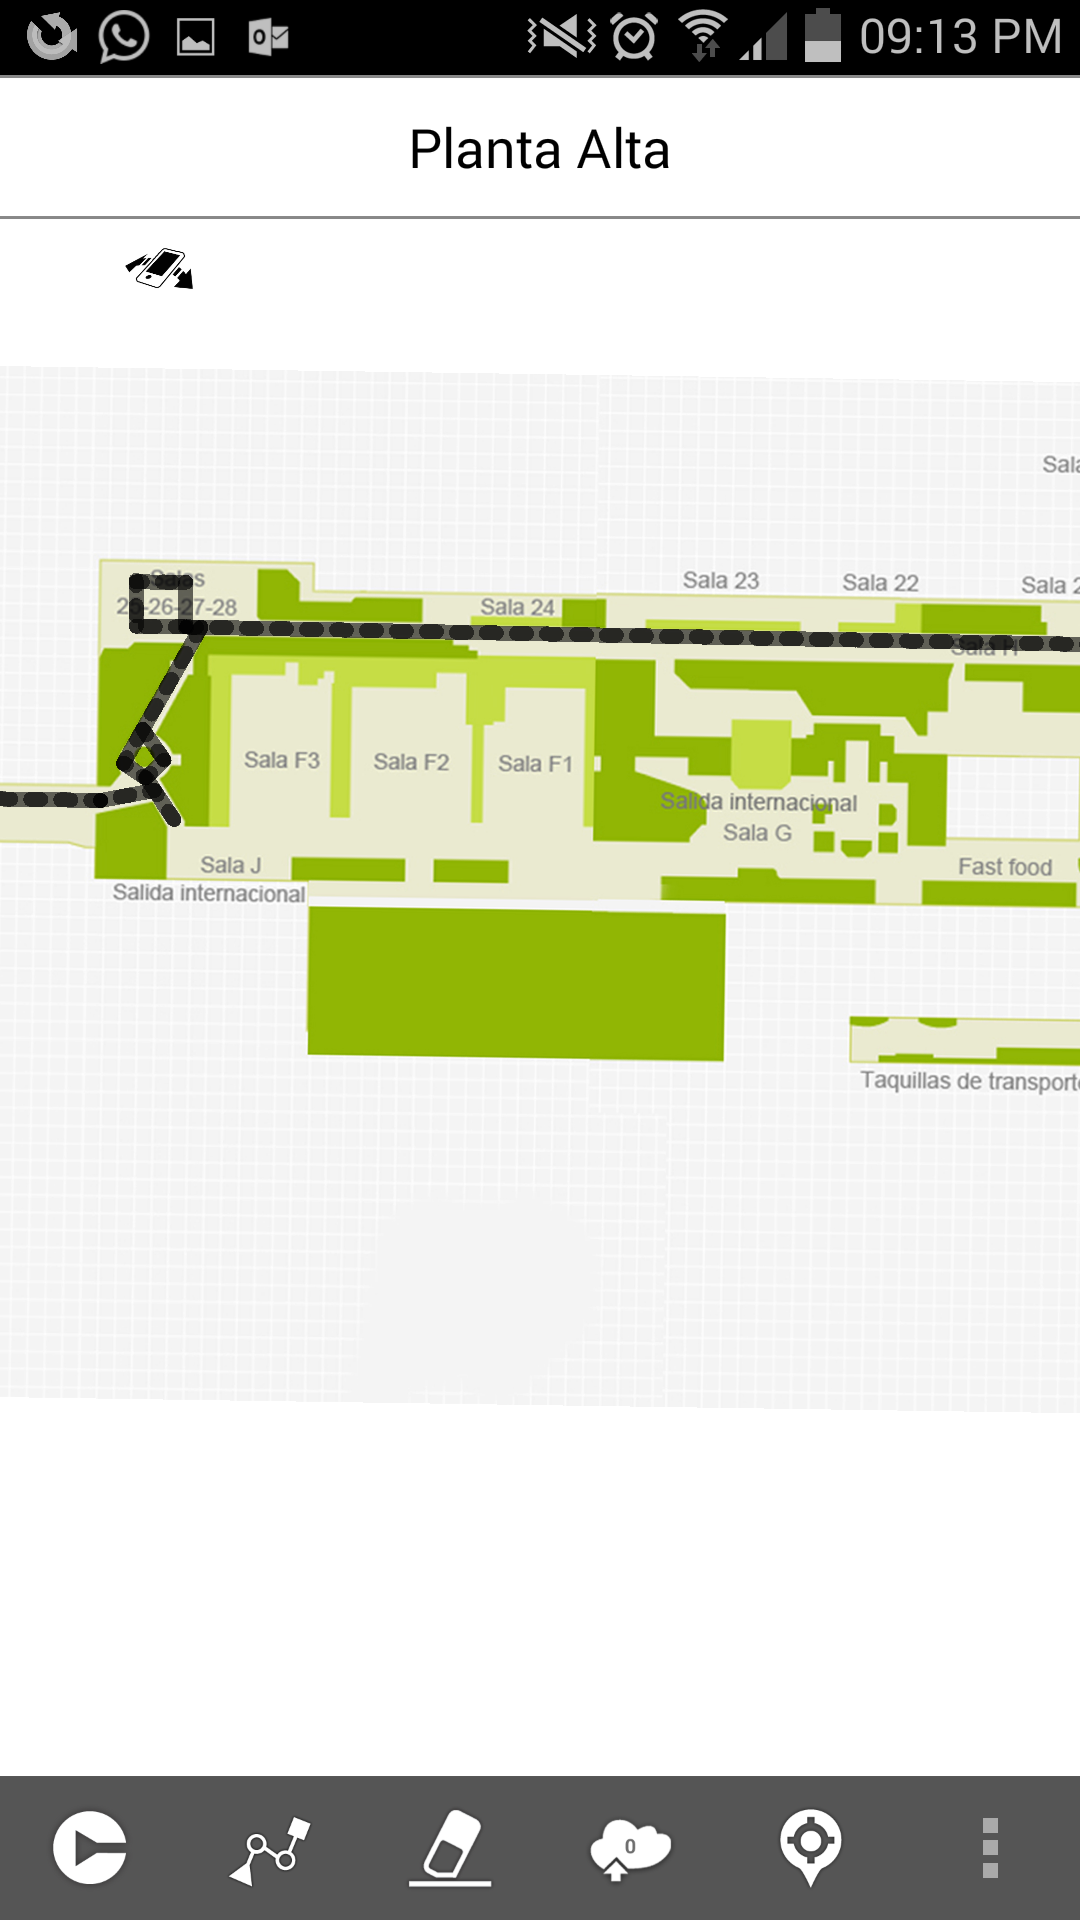
\includegraphics[width=0.5\textwidth]{Figuras/inter.png}
		\rule{30em}{0.5pt}
	\caption[Prueba trayectoria dentro de salas de última espera]{Prueba trayectoria dentro de salas de última espera}
	\label{fig:vistaPruebaSUES}
\end{figure}
\clearpage


\begin{figure}[h]
	\centering
		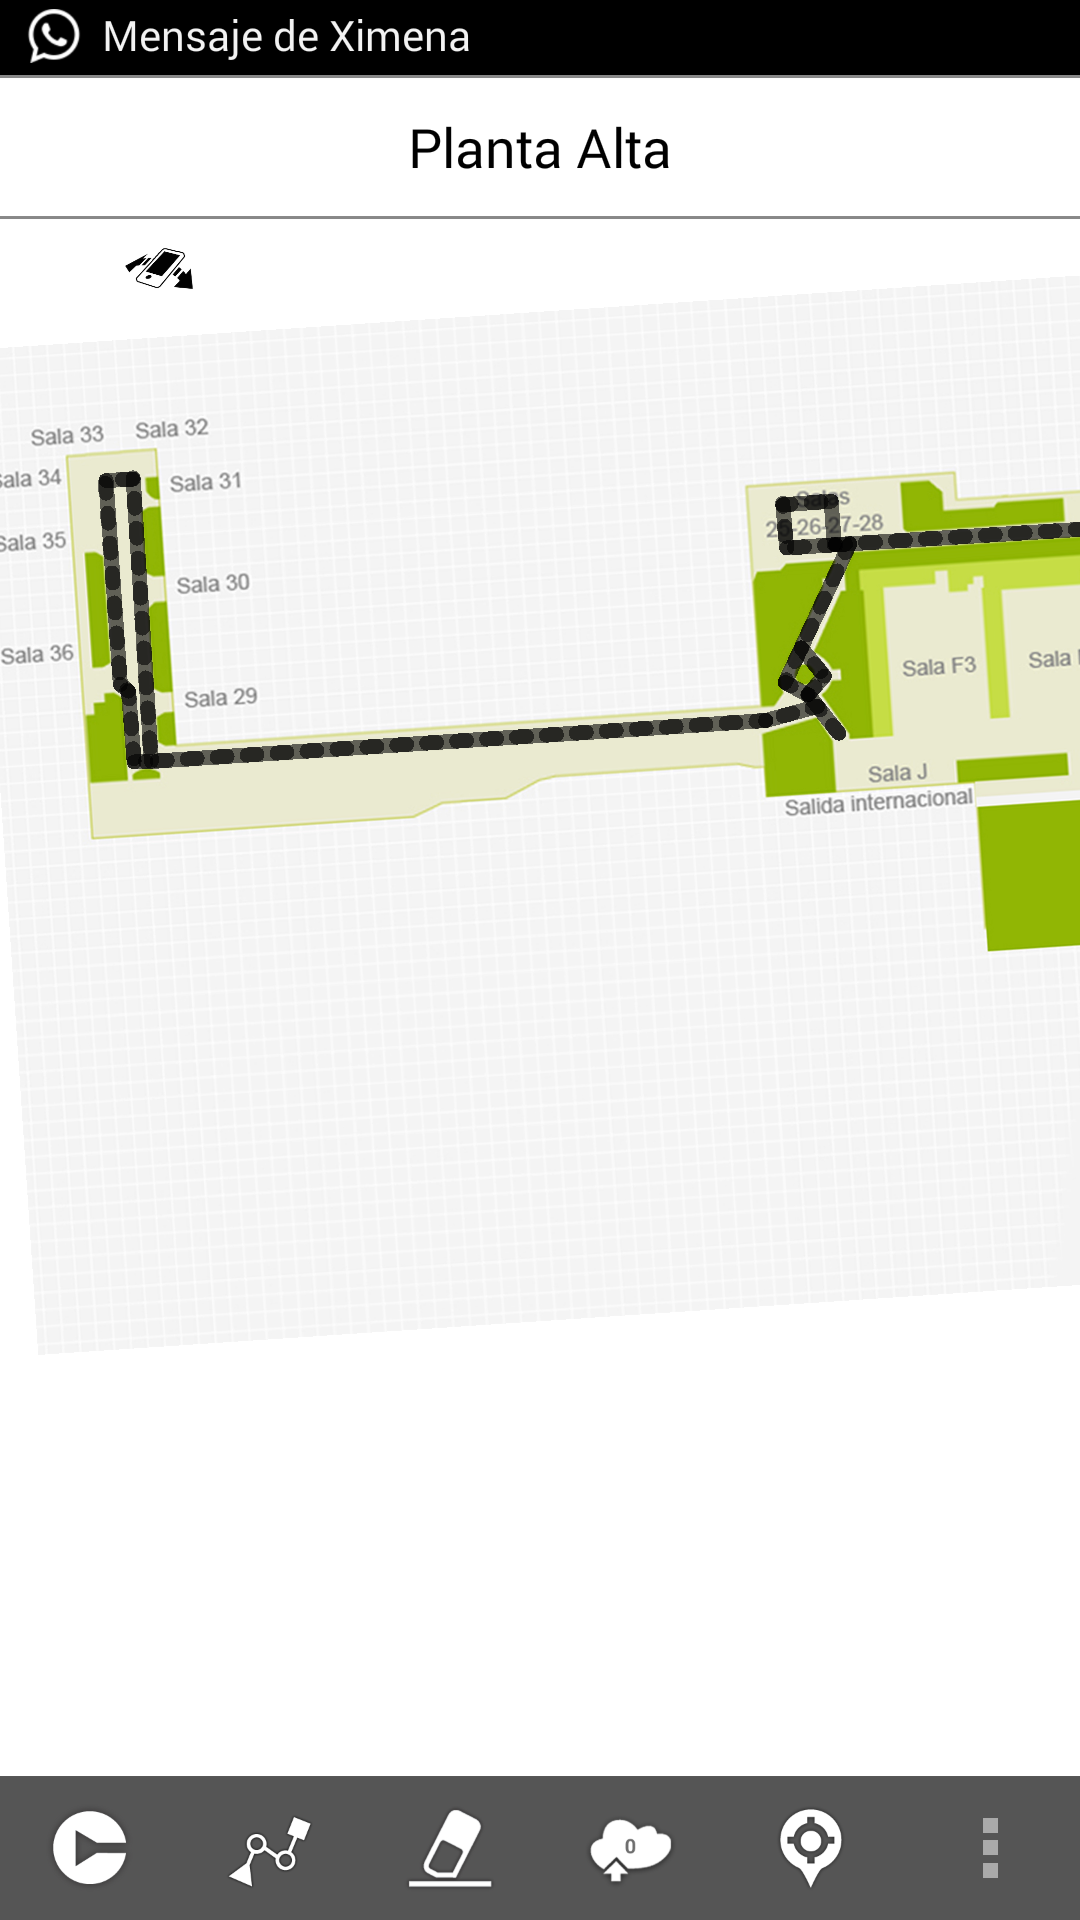
\includegraphics[width=0.5\textwidth]{Figuras/monarca.png}
		\rule{30em}{0.5pt}
	\caption[Prueba trayectoria pasillo monarca]{Prueba trayectoria pasillo monarca}
	\label{fig:vistaPruebaMonarca}
\end{figure}
\clearpage

\subsection{Concurrencia}
Se realizaron pruebas de cuantos usuarios soportaba al mismo tiempo la aplicación en la cual se necesito obtener un conjunto de 
dispositivos móviles que nos ayudarán a cumplir esta tarea. Se pudieron obtener 10 dispositivos entre los que se encuetran los siguientes: 

\begin{itemize}
\item Samsung Galaxy V Duos SM-G313HZ.
\item Sony Xperia E3 4G LTE.
\item Samsung Galaxy Ace 4 Lite Duos SM-G313M.
\item Samsung Galaxy S4 LTE-A GT-i9506.
\item Samsung Galaxy S5 Plus SM-G901F.
\item Sony Xperia M2 Aqua.
\item Motorola Moto E.
\end{itemize}

La siguiente tabla \ref{tab:pruebasConcurrencia} muestra los tiempos de respuesta por cada petición que se realizaba al servicio de 
hoteles y vuelos así como la respuesta a la localización dentro del AICM.

\definecolor{blanco}{RGB}{255,255,255}

\begin{table}[h]
	\begin{center}
		\begin{tabular}{|>{\color{blanco}}c|>{\color{blanco}}c|>{\color{blanco}}c|>{\color{blanco}}c|}
			\hline \rowcolor[RGB]{51,153,255} 
				{\bf Dispositivo} & 
				{\bf Tiempo de respuesta} &
				{\bf Localización AICM} &
				{\bf Interfaz} 
				\\
			\hline 
				\multicolumn{1}{|m{4.0cm}|}{\centering Samsung Galaxy V Duos SM-G313HZ} &
				\multicolumn{1}{m{4.0cm}|}{\centering 7 segundos} &
				\multicolumn{1}{m{3.5cm}|}{\centering 
\includegraphics[width=7mm, height=7mm]{Figuras/palomita.png}}&
				\multicolumn{1}{m{2.0cm}|}{\centering 
\includegraphics[width=7mm, height=7mm]{Figuras/feliz.png}}\\
      		\hline \rowcolor[RGB]{240,248,255} 
      				\multicolumn{1}{|m{4.0cm}|}{\centering Sony Xperia E3 4G LTE} &
				\multicolumn{1}{m{4.0cm}|}{\centering 9 segundos} &
				\multicolumn{1}{m{3.5cm}|}{\centering 
\includegraphics[width=7mm, height=7mm]{Figuras/palomita.png}} &
				\multicolumn{1}{m{2.0cm}|}{\centering 
\includegraphics[width=7mm, height=7mm]{Figuras/feliz.png}}\\
		\hline 
				\multicolumn{1}{|m{4.0cm}|}{\centering Samsung Galaxy Ace 4 Lite Duos SM-G313M.} &
				\multicolumn{1}{m{4.0cm}|}{\centering 7.1 segundos} &
				\multicolumn{1}{m{3.5cm}|}{\centering 
\includegraphics[width=7mm, height=7mm]{Figuras/palomita.png}}&
				\multicolumn{1}{m{2.0cm}|}{\centering 
\includegraphics[width=7mm, height=7mm]{Figuras/serio.png}}\\
      		\hline \rowcolor[RGB]{240,248,255} 
      				\multicolumn{1}{|m{4.0cm}|}{\centering Samsung Galaxy S4 LTE-A GT-i9506 (A)} &
				\multicolumn{1}{m{4.0cm}|}{\centering 7.6 segundos} &
				\multicolumn{1}{m{3.5cm}|}{\centering 
\includegraphics[width=7mm, height=7mm]{Figuras/palomita.png}}&
				\multicolumn{1}{m{2.0cm}|}{\centering 
\includegraphics[width=7mm, height=7mm]{Figuras/feliz.png}}\\
		\hline 
				\multicolumn{1}{|m{4.0cm}|}{\centering Samsung Galaxy S4 LTE-A GT-i9506 (B)} &
				\multicolumn{1}{m{4.0cm}|}{\centering 8 segundos} &
				\multicolumn{1}{m{3.5cm}|}{\centering 
\includegraphics[width=7mm, height=7mm]{Figuras/palomita.png}}&
				\multicolumn{1}{m{2.0cm}|}{\centering 
\includegraphics[width=7mm, height=7mm]{Figuras/feliz.png}}\\
      		\hline \rowcolor[RGB]{240,248,255} 
      				\multicolumn{1}{|m{4.0cm}|}{\centering Samsung Galaxy S5 Plus SM-G901F} &
				\multicolumn{1}{m{4.0cm}|}{\centering 6.3 segundos} &
				\multicolumn{1}{m{3.5cm}|}{\centering 
\includegraphics[width=7mm, height=7mm]{Figuras/palomita.png}}&
				\multicolumn{1}{m{2.0cm}|}{\centering 
\includegraphics[width=7mm, height=7mm]{Figuras/feliz.png}}\\
		\hline 
				\multicolumn{1}{|m{4.0cm}|}{\centering Sony Xperia M2 Aqua (A)} &
				\multicolumn{1}{m{4.0cm}|}{\centering 8.2 segundos} &
				\multicolumn{1}{m{3.5cm}|}{\centering 
\includegraphics[width=7mm, height=7mm]{Figuras/palomita.png}}&
				\multicolumn{1}{m{2.0cm}|}{\centering 
\includegraphics[width=7mm, height=7mm]{Figuras/feliz.png}}\\
      		\hline \rowcolor[RGB]{240,248,255} 
      				\multicolumn{1}{|m{4.0cm}|}{\centering Sony Xperia M2 Aqua (B)} &
				\multicolumn{1}{m{4.0cm}|}{\centering 8.7 segundos} &
				\multicolumn{1}{m{3.5cm}|}{\centering 
\includegraphics[width=7mm, height=7mm]{Figuras/palomita.png}}&
				\multicolumn{1}{m{2.0cm}|}{\centering 
\includegraphics[width=7mm, height=7mm]{Figuras/feliz.png}}\\
		\hline 
				\multicolumn{1}{|m{4.0cm}|}{\centering Motorola Moto E} &
				\multicolumn{1}{m{4.0cm}|}{\centering 9.3} &
				\multicolumn{1}{m{3.5cm}|}{\centering 
\includegraphics[width=7mm, height=7mm]{Figuras/palomita.png}}&
				\multicolumn{1}{m{2.0cm}|}{\centering 
\includegraphics[width=7mm, height=7mm]{Figuras/feliz.png}}\\
      		
		\hline 
    	\end{tabular}
	\end{center}
	\caption[Pruebas del módulo Concurrencia]{Pruebas del módulo Concurrencia} 
	\label{tab:pruebasConcurrencia}
\end{table}